\chapter{MATLAB code}\label{ch:matlab}

\lstinputlisting[style=matlab-editor, caption={MATLAB code to import and identify system of order $nx$ using the command \mcode{n4sid}, before plotting estimated response together with the actual response of the system}, label=lst:identification]{MATLAB/identification_general.m}

\chapter{Simulink diagrams}\label{ch:simulink}

\begin{figure}[ht!]
	\centering
	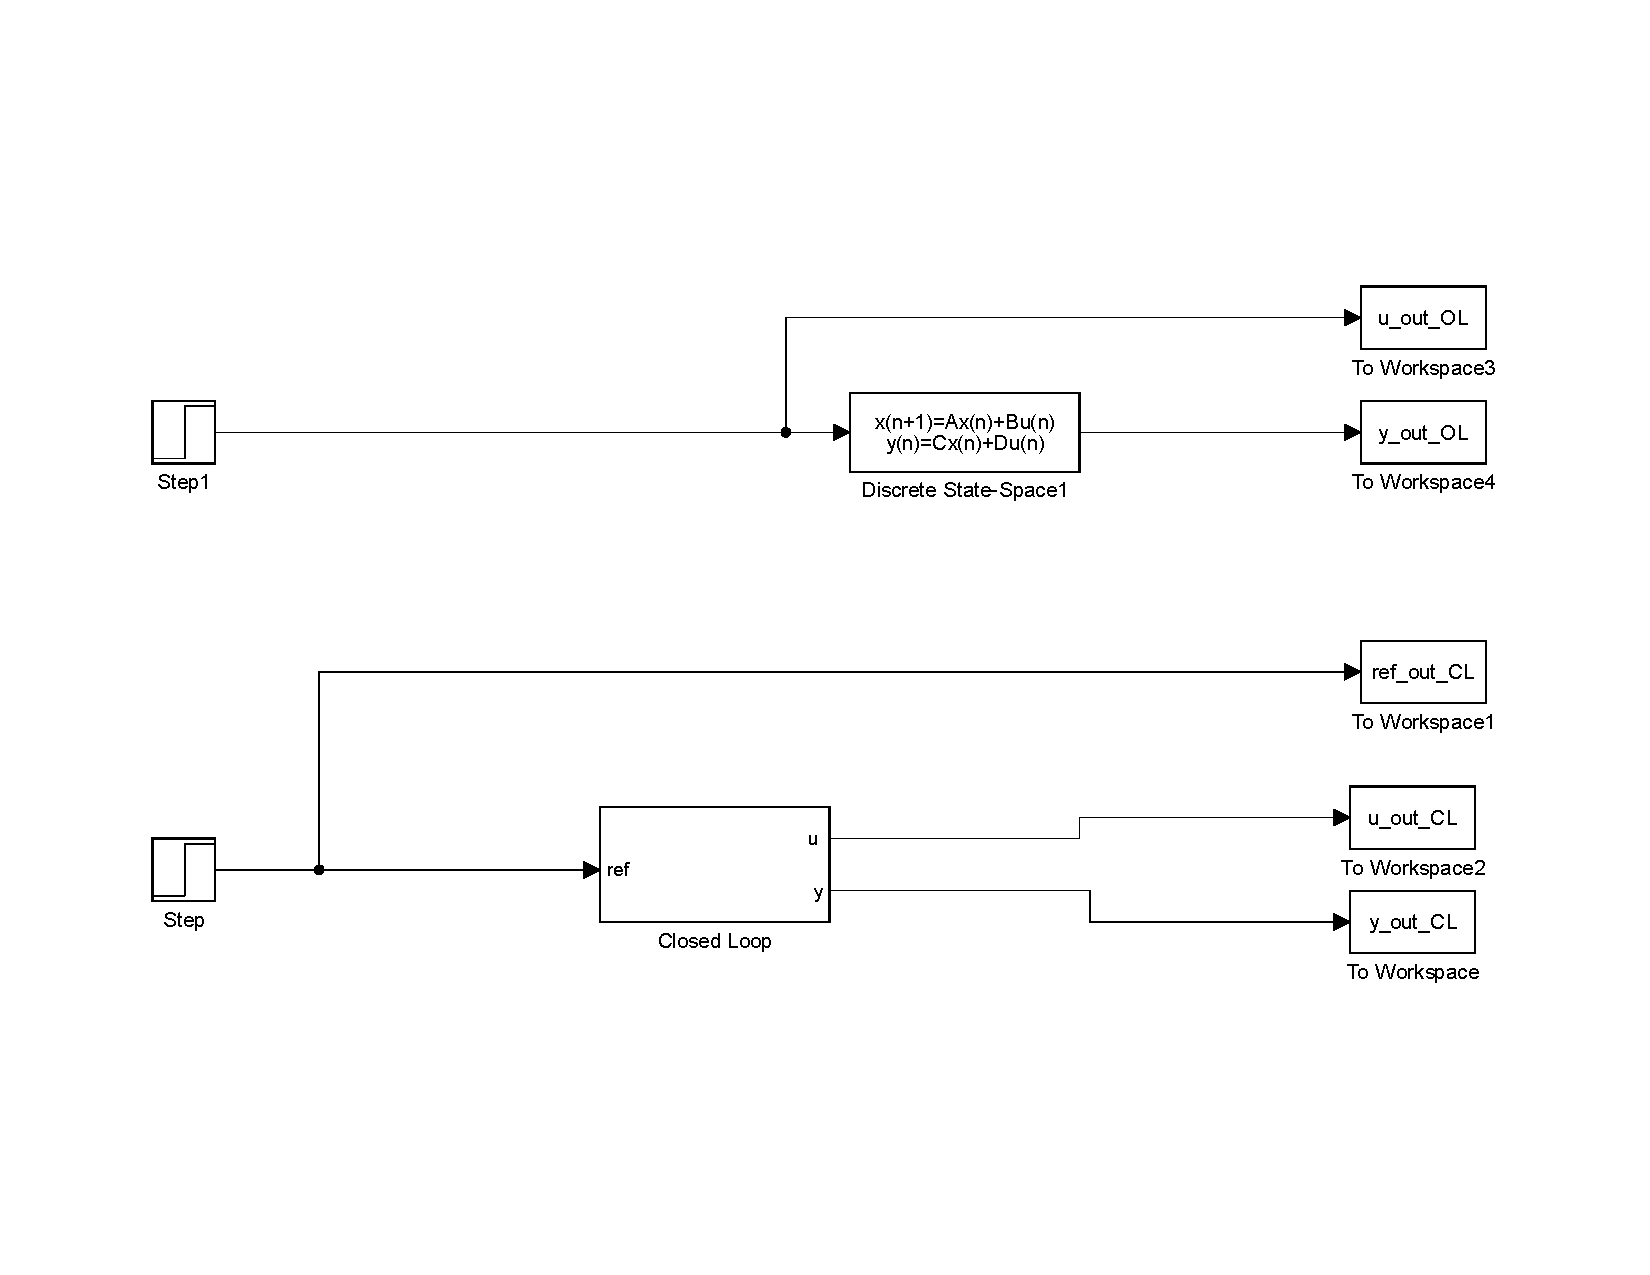
\includegraphics[width=0.95\textwidth]{fig/simulink/system_general.pdf}
	\caption{General Simulink diagram of identified system with both open and closed loop system}
	\label{fig:system_simulink}
\end{figure}

\begin{figure}[ht!]
	\centering
	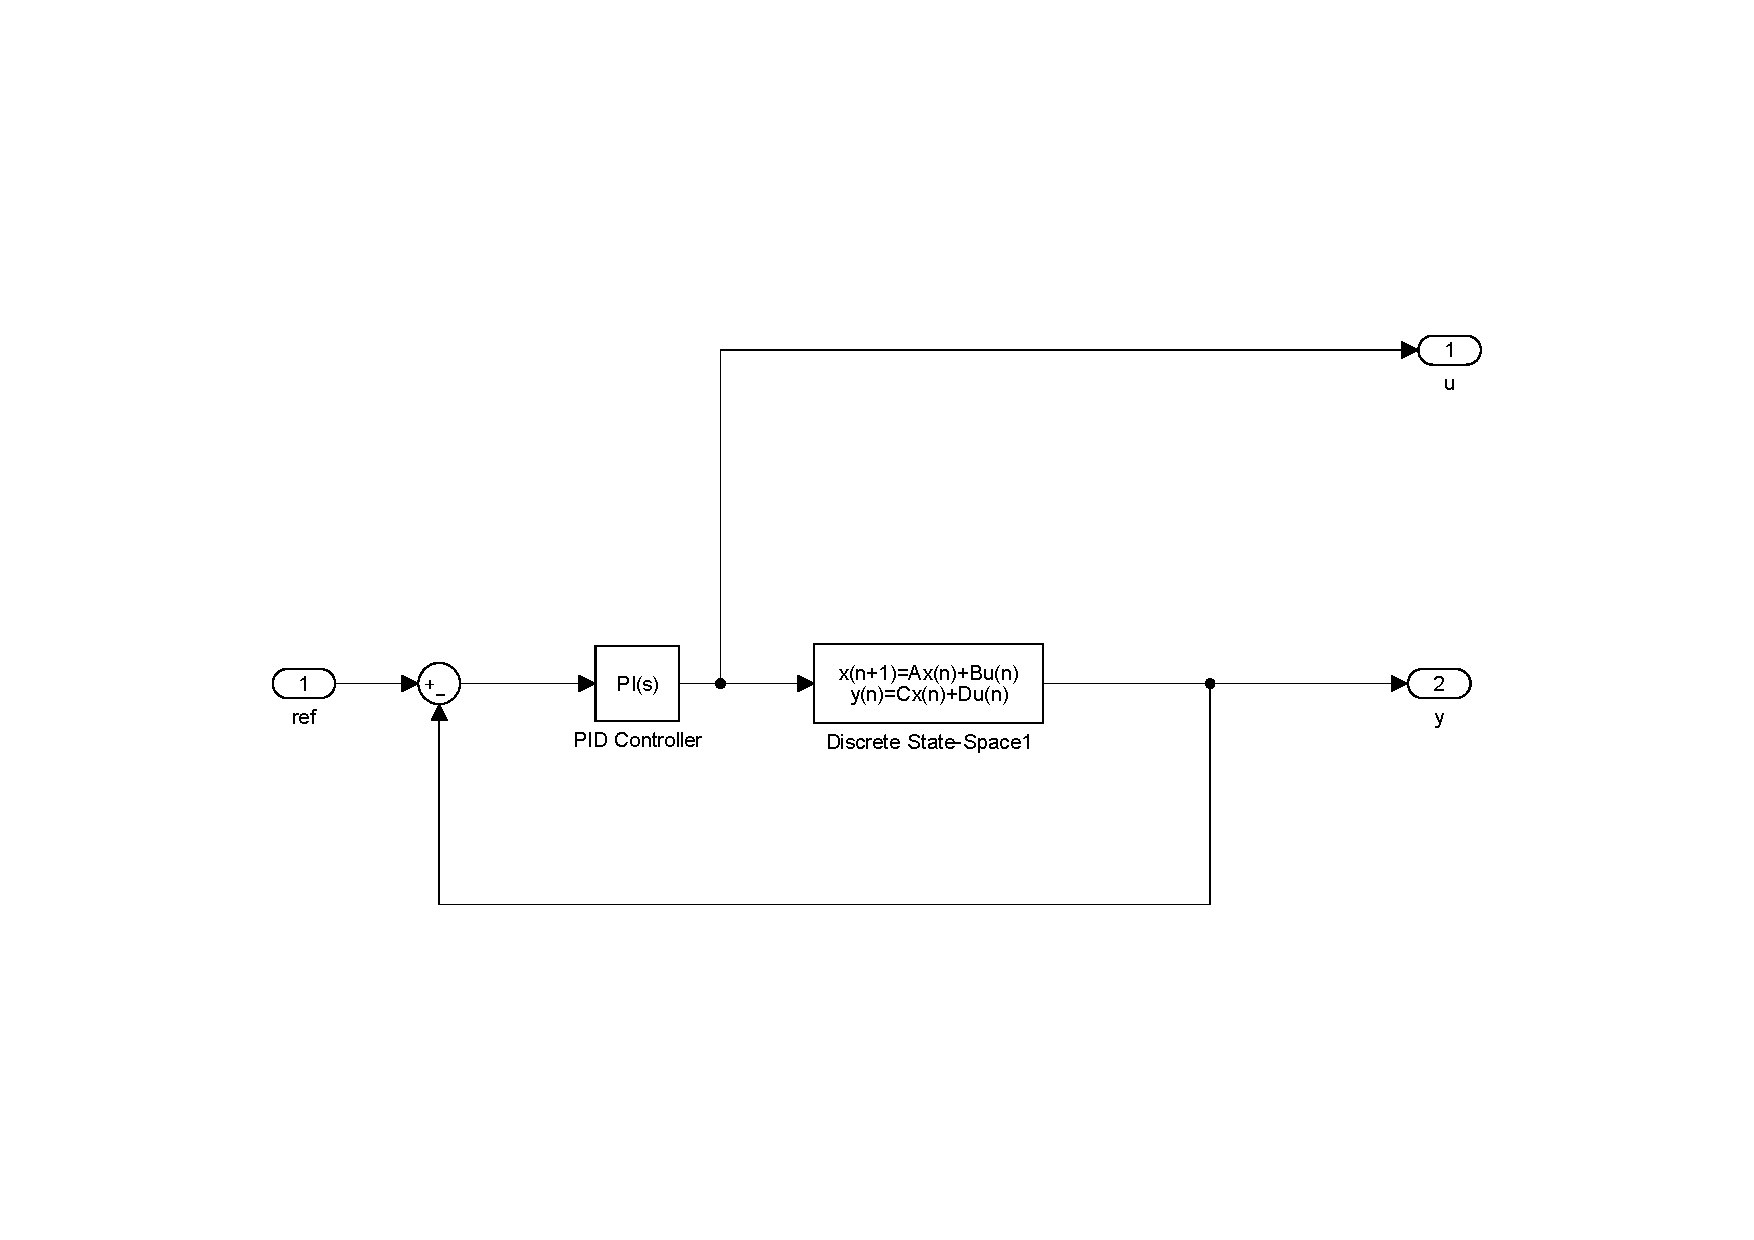
\includegraphics[width=0.95\textwidth]{fig/simulink/system_CL.pdf}
	\caption{Detailed diagram of the closed loop part of the system}
	\label{fig:system_CL}
\end{figure}

\chapter{MCL-scripts}\label{ch:mcl}

\lstinputlisting[caption = {MCL script to run system for two hours and performing three steps to evaluate performance of controller}, label = {lst:lc1016_tuned}]{K-Spice/ButaneSplitter/TimeLines/ButaneSplitter/ExplorerFiles/ProcessModel/lc1016_tuned.mcl}

\lstinputlisting[caption = {MCL script to run system for five hours and performing several step changes in controller output of controller  \texttt{24\_TC1088}.}, label = {lst:tc1088_exp}]{K-Spice/ButaneSplitter/TimeLines/ButaneSplitter/ExplorerFiles/ProcessModel/TemperatureExperiment.mcl}